\documentclass{article}
\usepackage[utf8]{inputenc}
\usepackage[russian]{babel}
\usepackage[14pt]{extsizes}
\usepackage{xcolor}
\usepackage{graphicx}
\usepackage{hyperref}
\usepackage{listings}
\usepackage{float}
\usepackage[left=2.5cm, right=1.5cm, vmargin=2.5cm]{geometry}

\fontsize{12}{17}
% \usepackage{indentfirst}

%Syntax highlights
\lstset {language = C++, backgroundcolor = \color{blue!5}, basicstyle = \footnotesize, commentstyle={}, texcl=true}

%Links color
\definecolor{linkcolor}{HTML}{0000BB}
\definecolor{urlcolor}{HTML}{0000BB}
\hypersetup{pdfstartview=FitH,  linkcolor = linkcolor, urlcolor=urlcolor, colorlinks=true}
\pagestyle{empty}

\begin{document}
\begin{center}
  \Large{Санкт-Петербургский Государственный Университет\\
  Аэрокосмического Приборостроения}\\
  \vspace{9cm}
  \LARGE{Курсовая Работа}\\
  \vspace{1cm}
  \textbf{\HugeАлгоритм Фано}\\
  \vspace{5cm}
\end{center}


\vspace{1em}
\begin{tabular}{ccc}
  Преподаватель & \hspace{8cm} & Иванов Д.О.\\
  Студент & \hspace{9.5cm} & Сирота А.В. 
\end{tabular}

\vspace{1em}

\vfill
\begin{center}
Санкт-Петербург 2016
\end{center}

\newpage

\pagestyle{plain}
\tableofcontents 

\newpage
\section {Постановка задачи}


Целью этой курсовой работы является разработка программы, которая будет иметь следующий функционал:

\begin{enumerate}
  \item Кодирование файла
  
  \begin{itemize}
    \item Побайтовый анализ кодируемого файла
    \item Построение кодов кодирования по алгоритму Фано
    \item Создание закодированного файла
  \end{itemize}
  
  \item Декодирование файла
  
  \begin{itemize}
    \item Анализ закодированного файла
    \item Создание раскодированного файла, который полностью идентичен файлу до кодировки
  \end{itemize}
\end{enumerate}

\newpage
\section{Алгоритм}
Алгоритм Шеннона --- Фано --- один из первых алгоритмов сжатия, который впервые сформулировали 
американские учёные Шеннон и Роберт Фано. Он был независимо друг от друга разработан Шенноном 
(публикация «Математическая теория связи», 1948 год) и, позже, Фано (опубликовано как технический отчёт).

\subsection{Основные сведения}

Алгоритм Шеннона --- Фано относится к вероятностным методам сжатия. 
\textit{Вероятностный метод сжатия} --- это метод, основанный на частоте встречаемости символа в тексте.

Подобно алгоритму Хаффмана, алгоритм Шеннона — Фано использует избыточность сообщения, 
заключённую в неоднородном распределении частот символов его первичного алфавита, 
то есть заменяет коды более частых символов короткими двоичными последовательностями, 
а коды более редких символов --- более длинными двоичными последовательностями. 

Коды, построенные по этому алгоритму, являются префиксными. Это необходимое условие 
однозначного декодирования. Префиксным называют код, удовлетворяющий условию Фано: 
если в код входит слово a, то для любой непустой строки b слова ab в коде не существует.

Например, код, состоящий из слов 0, 10 и 11, является префиксным, и сообщение
$$
01001101110
$$
можно разбить на слова единственным образом:
$$
0\quad10\quad0\quad11\quad0\quad11\quad10
$$

Код, состоящий из слов 0, 10, 11 и 100, префиксным не является, и то же 
сообщение можно трактовать несколькими способами:
$$
0\quad10\quad0\quad11\quad0\quad11\quad10
$$$$
0\quad100\quad11\quad0\quad11\quad10
$$

Префиксные коды наглядно могут быть представлены с помощью кодовых деревьев. 
Если ни один узел кодового дерева не является вершиной данного кода, то он обладает 
свойствами префикса. Узлы дерева, которые не соединяются с другими, называются конечными. 
Комбинации, которые им соответствуют, являются кодовыми комбинациями префиксного кода.

\newpage
\subsection{Основные этапы}
Так выглядит алгоритм Фано в общем виде:
\begin{enumerate}
 \item Символы первичного алфавита m1 выписывают по убыванию вероятностей.
 \item Символы полученного алфавита делят на две части, суммарные вероятности 
 символов которых максимально близки друг другу.
 \item В префиксном коде для первой части алфавита присваивается двоичная цифра «0», 
 второй части --- «1».
 \item Полученные части рекурсивно делятся и их частям назначаются соответствующие 
 двоичные цифры в префиксном коде.\\
\end{enumerate}
Пример построения кодов по алгоритму Фано показан на рис. \ref{codesex}. Пример построения кодов.

\begin{figure}[H]
  \center{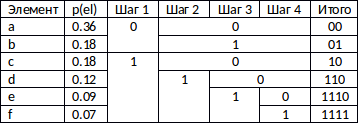
\includegraphics[height=10em]{codesex.png}}
  \caption{Пример построения кодов\label{codesex}}
\end{figure}


\newpage
\subsection{Алгоритм вычисления кодов}

Код Шеннона — Фано строится с помощью дерева. Построение этого дерева начинается от корня. 
Всё множество кодируемых элементов соответствует корню дерева (вершине первого уровня). 
Оно разбивается на два подмножества с примерно одинаковыми суммарными вероятностями. 

Эти подмножества соответствуют двум вершинам второго уровня, которые соединяются с корнем. 
Далее каждое из этих подмножеств разбивается на два подмножества с примерно одинаковыми 
суммарными вероятностями. Им соответствуют вершины третьего уровня. 

Если подмножество содержит 
единственный элемент, то ему соответствует концевая вершина кодового дерева; такое подмножество 
разбиению не подлежит.

Подобным образом поступаем до тех пор, пока не получим все концевые 
вершины. Ветви кодового дерева размечаем символами 1 и 0. 

На рис. \ref{tree} представлен пример 
построения кодового дерева. Каждой букве в соответствие поставлена встречаемость в кодируемом тексте.

\begin{figure}[H]
  \center{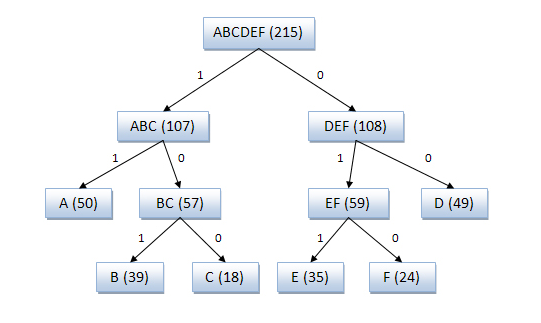
\includegraphics[height=20em]{tree.png}}
  \caption{Построение кодового дерева\label{tree}}
\end{figure}

\newpage
Ниже представлен псевдокод рекурсивной функции, которая осуществляет построение бинарного дерева и вычисление кодов.
\begin{lstlisting}
createCodeTree(begin, end, elements){
  //Если множество содержит один элемент, ничего не делать
  if(end == begin){
    return;
  }
  
  //Найти точку деления группы на подгруппы
  int point = findDividePoint(begin, end);
  
  //Добавить элементам первой подгруппы 0 в код
  for(int i = begin; i < point; i++){
    elements[i].code += "0";
  }
  
  //Добавить элементам второй подгруппы 1 в код
  for(int i = point; i < end; i++){
    elements[i].code += "1";
  }
  
  //Если в подгруппах > 1 элемента, делить дальше
  if(begin + 1 < point){
    createBranch(begin, point);
  }
  if(point + 1 < end){
    createBranch(point, end);
  }
}
\end{lstlisting}

При построении кода Шеннона --- Фано разбиение множества элементов может быть произведено, вообще 
говоря, несколькими способами. Выбор разбиения на уровне n может ухудшить варианты разбиения на 
следующем уровне (n~+~1) и привести к неоптимальности кода в целом. 

Другими словами, 
оптимальное поведение на каждом шаге пути ещё не гарантирует оптимальности всей совокупности действий. 
Поэтому код Шеннона~---~Фано не является оптимальным в общем смысле, хотя и дает оптимальные 
результаты при некоторых распределениях вероятностей. 

Для одного и того же распределения вероятностей 
можно построить, вообще говоря, несколько кодов Шеннона --- Фано, и все они могут дать различные 
результаты. Если построить все возможные коды Шеннона --- Фано для данного распределения вероятностей, 
то среди них будут находиться и все коды Хаффмана, то есть оптимальные коды.

Для примера, рассмотрим последовательность в табл. \ref{hafacomp}. 
\begin{table}
  \begin{center}
    \begin{tabular}{|c|c|c|c|}
      \hline
      Символ & Встречаемость & Код Хаффмана & Код Шеннона --- Фано \\
      \hline
      a & 14 & 0 & 00 \\
      \hline
      b & 7 & 111 & 01 \\
      \hline
      c & 5 & 101 & 10 \\
      \hline
      d & 5 & 110 & 110 \\
      \hline
      e & 4 & 100 & 111 \\
      \hline
    \end{tabular}
    \caption{Сравнение кодов Хаффмана и Шеннона --- Фано\label{hafacomp}}
  \end{center}
\end{table}
Метод Хаффмана сожмёт её до 77 бит, а вот Шеннона --- Фано до 79 бит.

\section{Руководство пользователя}

Программа fano осуществляет сжатие текстовых файлов по алгоритму Шеннона – Фано.\\

Репозиторий на GitHub: \fbox{\url{https://github.com/nukefluke/fano-algorithm}}

\vspace{2em}
Программа запускается из консоли, команда запуска выглядит так:

\begin{lstlisting}
  $ fano <mode> <input> [-o <output>]
\end{lstlisting}

Параметр mode отвечает за режим работы программы. Список режимов приведён в табл. \ref{modes}.

\begin{table}
 \begin{center}
  \begin{tabular}{|c|c|c|}
   \hline
   Режим & Описание & Входной файл\\
   \hline
    & Режим кодирования.  & \\ 
   -e & В выходной файл записывается & Любой \\
    & шапка с таблицей кодировки и закодированный файл. & \\
   \hline
    & Режим декодирования. & \\
   -d & Выходной файл является точной копией файла, & *.fano\\ 
    & который был закодирован. & \\
   \hline
  \end{tabular}

 \end{center}
  \caption{Режимы работы программы\label{modes}}
\end{table}


Параметром input указывается путь ко входному файлу.

Параметр output устанавливает имя выходного файла. Если параметр не указан, имя файла будет сгенерировано автоматически.

\subsection{Примеры команд запуска}
Закодировать файл input.txt. Выходной файл будет иметь название input.txt.fano:
\$ fano -e input.txt 
Декодировать файл input.fano и сохранить как decoded.dat:
\$ fano –d input.fano –o decoded.dat

\subsection{Производительность} 
\subsection{Эффективность}
Результаты тестов программы представлены в
\end{document}